\chapter{Problématiques émergentes}

\section{Orientations de recherche}

Dans ce mémoire, nous avons décris diverses modèles et principes de conception
d'un système sensible au contexte et présenté une multitude d'intergiciels et
d'approches distribuées pour simplifier la configuration d'application sensibles
au contexte. De cet état de l'art se dégagent plusieurs problématiques dans le
développement d'un système de configuration basé sur le contexte auxquelles nous
nous tenterons d'apporter une solution. Voici les trois les plus pertinentes :

\subsection{Integiciel et détails d'implémentation}

Le besoin d'un nouvel intergiciel se fait sentir du coté de l'implémentation.
Les technologies intergicielles actuelles ne sont pas adaptées pour le prise en
considération des restrictions imposées pas la mobilité et les systèmes
environementaux intelligents : connexions volatiles, traitements et restrictions
mémoire sur les périphériques mobiles, cannaux de communication étroits, écrans
réduits, mécanismes d'entrées restreintes, et la liste continue. Il existe
néamoins une gamme d'implémentations de systèmes sensible au contexte dans la
littérature avec quelques prototypes fonctionnels :

\begin{itemize}
    \item \textbf{Hydrogen} \cite{hofer_context-awareness_2003}: 
	    une architecture en trois couches.
    \item \textbf{Gaia} \cite{chetan_mobile_2005}: 
            une autre infrastructure intergicielle, etends les caractéristiques
	    génériques des systèmes d'exploitation pour y incorporer la
	    sensibilité au contexte.
    \item \textbf{CybreMinder} \cite{abowd_context-aware_2002}: 
	    un système sensible au contexte permettant de génerer des messages
	    de rappel.
    \item \textbf{Context Toolkit} \cite{dey_conceptual_2001}: 
	    une architecture basée sur les widgets.
\end{itemize}

\subsection{Représentation des informations de contexte}

La représentation des informations de contexte est une autre préocupation. Nous
avons présenté dans ce mémoire une approche basée sur les ontologie très
générique. Elle est basée sur quatre concepts fondamentaux : utilisateur,
environemment, plateforme et ressources. Actuellement, les ontologies sont
surtout utilisées pour permettre la communication entre les différents
périphériques dans le même réseau. Comme proposé par le ContextUML
\cite{sheng_contextuml:_2005}, le Langage de Modélisation Unifié (UML) peut
égalemment être utilisé pour modéliser le contexte. Ces modèles pourrait être
utilisés pour séparer la définition et l'information liée au contexte de
l'implémentation spécifique. Il existe d'autre caractéristiques qui font que
l'information de contexte est difficile à modéliser : comme abordé précédemment,
il est parfois nécéssaire de différencier une information statique d'une
information dynamique.

\subsection{Règles sémantiques}

Un autre domaine de recherche concernerait l'utilisation de règles pour exprimer
les comportemments souhaités en termes d'éléments de haut-niveau. Des langages
de définition de règles sont utilisés dans certains cas pour obtenir la
sensibilité au contexte. CRIME \cite{murphy_coordination_2007} par exemple, est
une implémentation prototypique du modèle Fact Space, qui est un langage de
coordination fournissant aux applications une vue de leur environement. Les
règles CRIME décrivent le comportemment des applications conformément à
l'information de contexte. CRIME traite également les déconnexions en invalidant
les faits et conclusions qui sont tirés des périphériques qui ne sont plus
disponibles dans l'environnement.

\section{Ontologie de contexte}

L'une des principales innovations à apporter dans les infrastructures
d'applications sensibles au contexte réside dans l'introduction d'une interface
présentant un niveau d'abstraction élevé. Cela permetterait de représenter la
connectivité des composants applicatifs avec les politiques de haut niveau qui
la régissent.  Cette couche doit rester simple d'utilisation pour les
développeurs d'applications, et le modèle améliorer simultanément
l'automatisation et la sécurité.

\section{Théorie de promesse}

Le modèle permettant la définition des politiques d'administration serait un
modèle orienté sur les ontologies et basé sur la théorie de la promesse.
Celle-ci s'appuie sur un contrôle évolutif des objets intelligents,
contrairement aux modèles impératifs plus traditionnels pensés comme des
systèmes de gestion descendants.  Dans ces derniers, le gestionnaire central
doit être informé des commandes de configuration des objets sous-jacents et de
l'état actuel de ces objets.

Au sein du contexte, le modèle fournit une série d'objets qui définissent
l'application. Les objets englobent les terminaux, les groupes de terminaux et
les politiques qui définissent leur relation.

L'infrastructure conçoit un modèle d'objet pour le déploiement d'applications,
ces dernières constituant le point central. Historiquement, les applications
étaient limitées par les capacités du réseau et par des configurations visant à
prévenir leur utilisation abusive. Des concepts tels que l'adressage, le VLAN et
la sécurité sont depuis toujours intimement liés, ce qui limite l'évolutivité et
la mobilité des applications. Alors que les applications sont redessinées pour
la mobilité et l'évolutivité web, cette approche traditionnelle empêche leur
déploiement rapide et homogène.

\subsection{Principes de fonctionnement}

\section{Algorithmes de consensus}

\subsection{Algorithme de Paxos}

\subsection{Algorithme de Raft}

Raft est un algorithme de consensus qui est conçu pour être facile à comprendre.
Il est équivalent à Paxos dans la tolérance aux pannes et en termes de
performance. La différence, c'est qu'il est décomposé en sous-problèmes
relativement indépendants, et il traite de manière rigoureuse toutes les pièces
majeures nécessaires pour obtenir un système cohérent.

Le consensus est un problème fondamental dans les systèmes distribués tolérants
aux pannes. Consensus implique de multiples serveurs acceptant des valeurs. Une
fois qu'ils atteignent une décision sur une valeur, cette décision est
définitive. Les algorithmes de consensus typiques  sont amenés à faire des
progrès lorque la majorité de leurs serveurs sont disponibles, par exemple, un
cluster de 5 serveurs peut continuer à fonctionner même si deux serveurs ne sont
plus disponibles. Si plusieurs serveurs échouent, ils cessent de faire des
progrès (mais ils ne retournerons jamais de valeurs érronées)

\section{Vue d'ensemble}

Comme on le voit \ref{archi}

\begin{figure}[ht!]
  \centering
  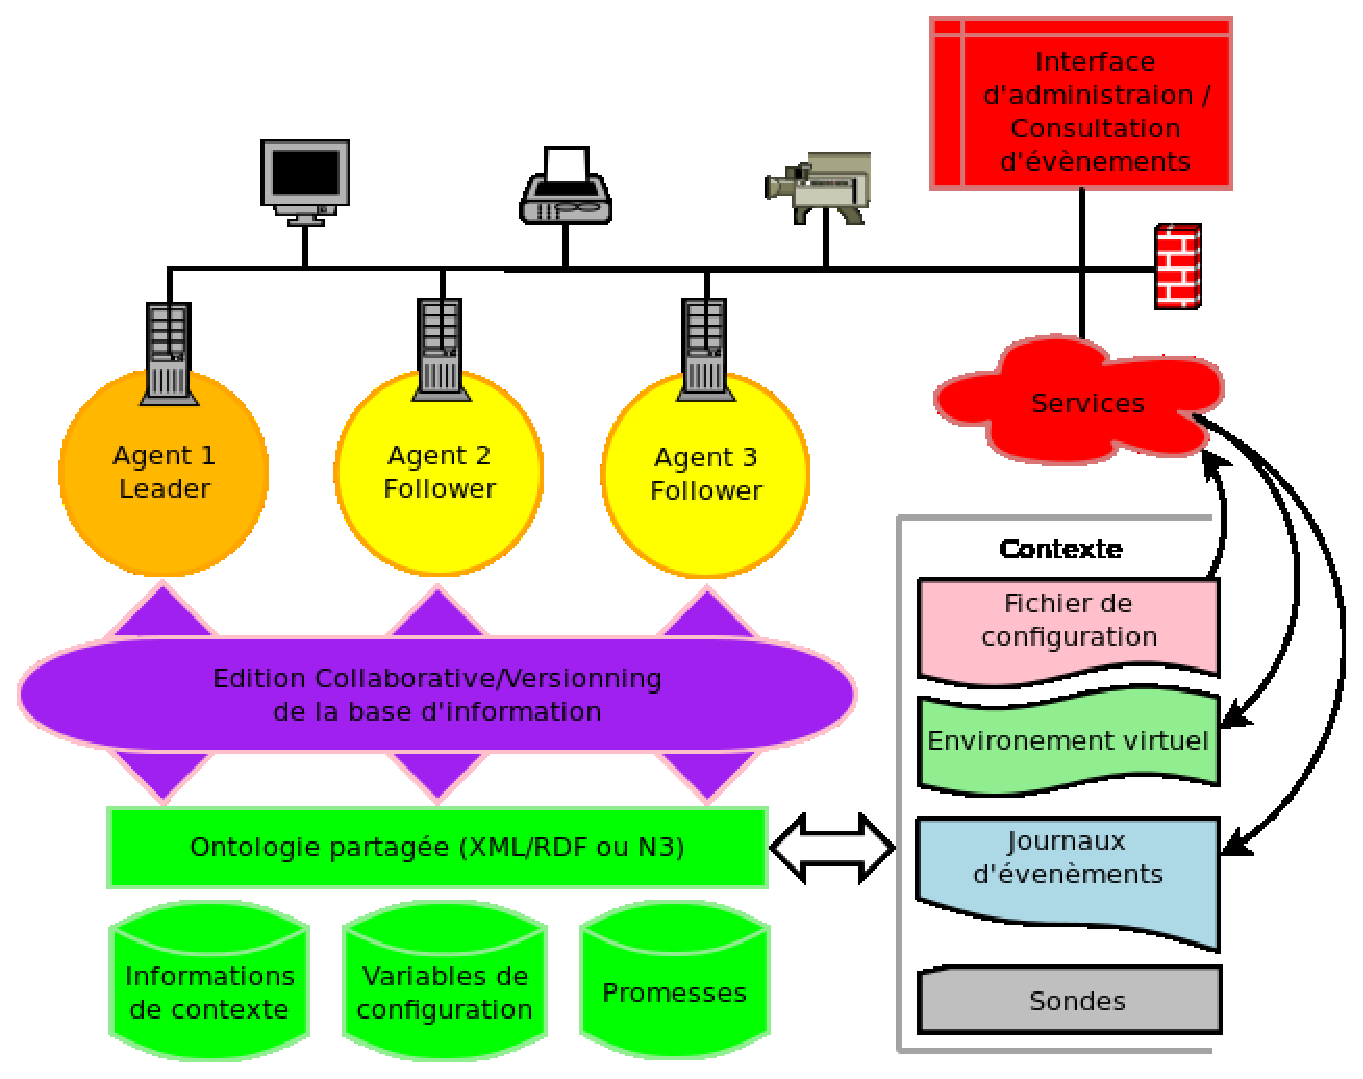
\includegraphics[width=90mm]{img/archi}
  \caption{Schéma d'implémentation du système multi-agents}
  \label{archi}
\end{figure}
